\section{Current Research Directions}

\begin{frame}
    \frametitle{A Splash of Differential Equations}

    What is an \textit{\textbf{Ordinary Differential Equation}}?

    \vline

    Imposition of a relationship between functions of a independent single variable and its derivatives.

    \vline

    e.g. Newton's Second Law of Motion (in 1 Dimension)

    \begin{equation}
        m \frac{d^2x}{dt^2} = F(x(t))
    \end{equation}

\end{frame}



\begin{frame}
    \frametitle{A Splash of Differential Equations}

    What is a \textit{\textbf{Partial Differential Equation}}?

    \vline

    Imposition of a relationship between functions of a multiple independent variables and their derivatives.

    \vline

    e.g. The Heat Equation (in 3D Cartesian Coordinates, $\Delta = \frac{d^2}{dx^2} + \frac{d^2}{dy^2} + \frac{d^2}{dz^2}$)

    \begin{equation}
        \frac{du}{dt} = \Delta u
    \end{equation}

    \vline

    Where $u(x, y, z, t)$.

\end{frame}

\begin{frame}
    \frametitle{Variational Methods for PDEs I}

    \begin{columns}

        \begin{column}{0.5\textwidth}

            Finite Element Method (FEM):

            \begin{enumerate}
                \item Meshes over volume.
                \item Results in sparse matrices.
                \item Requires explicit boundary conditions.
            \end{enumerate}
        \end{column}

        \begin{column}{0.5 \textwidth}
            Boundary Element Method (BEM):

            \begin{enumerate}
                \item Meshes over surface.
                \item Results in full matrices.
                \item Boundary conditions captured in formulation.
            \end{enumerate}
        \end{column}
    \end{columns}
\end{frame}

\begin{frame}
\frametitle{Variational Methods for PDEs II}
    Consider 2D problem:

    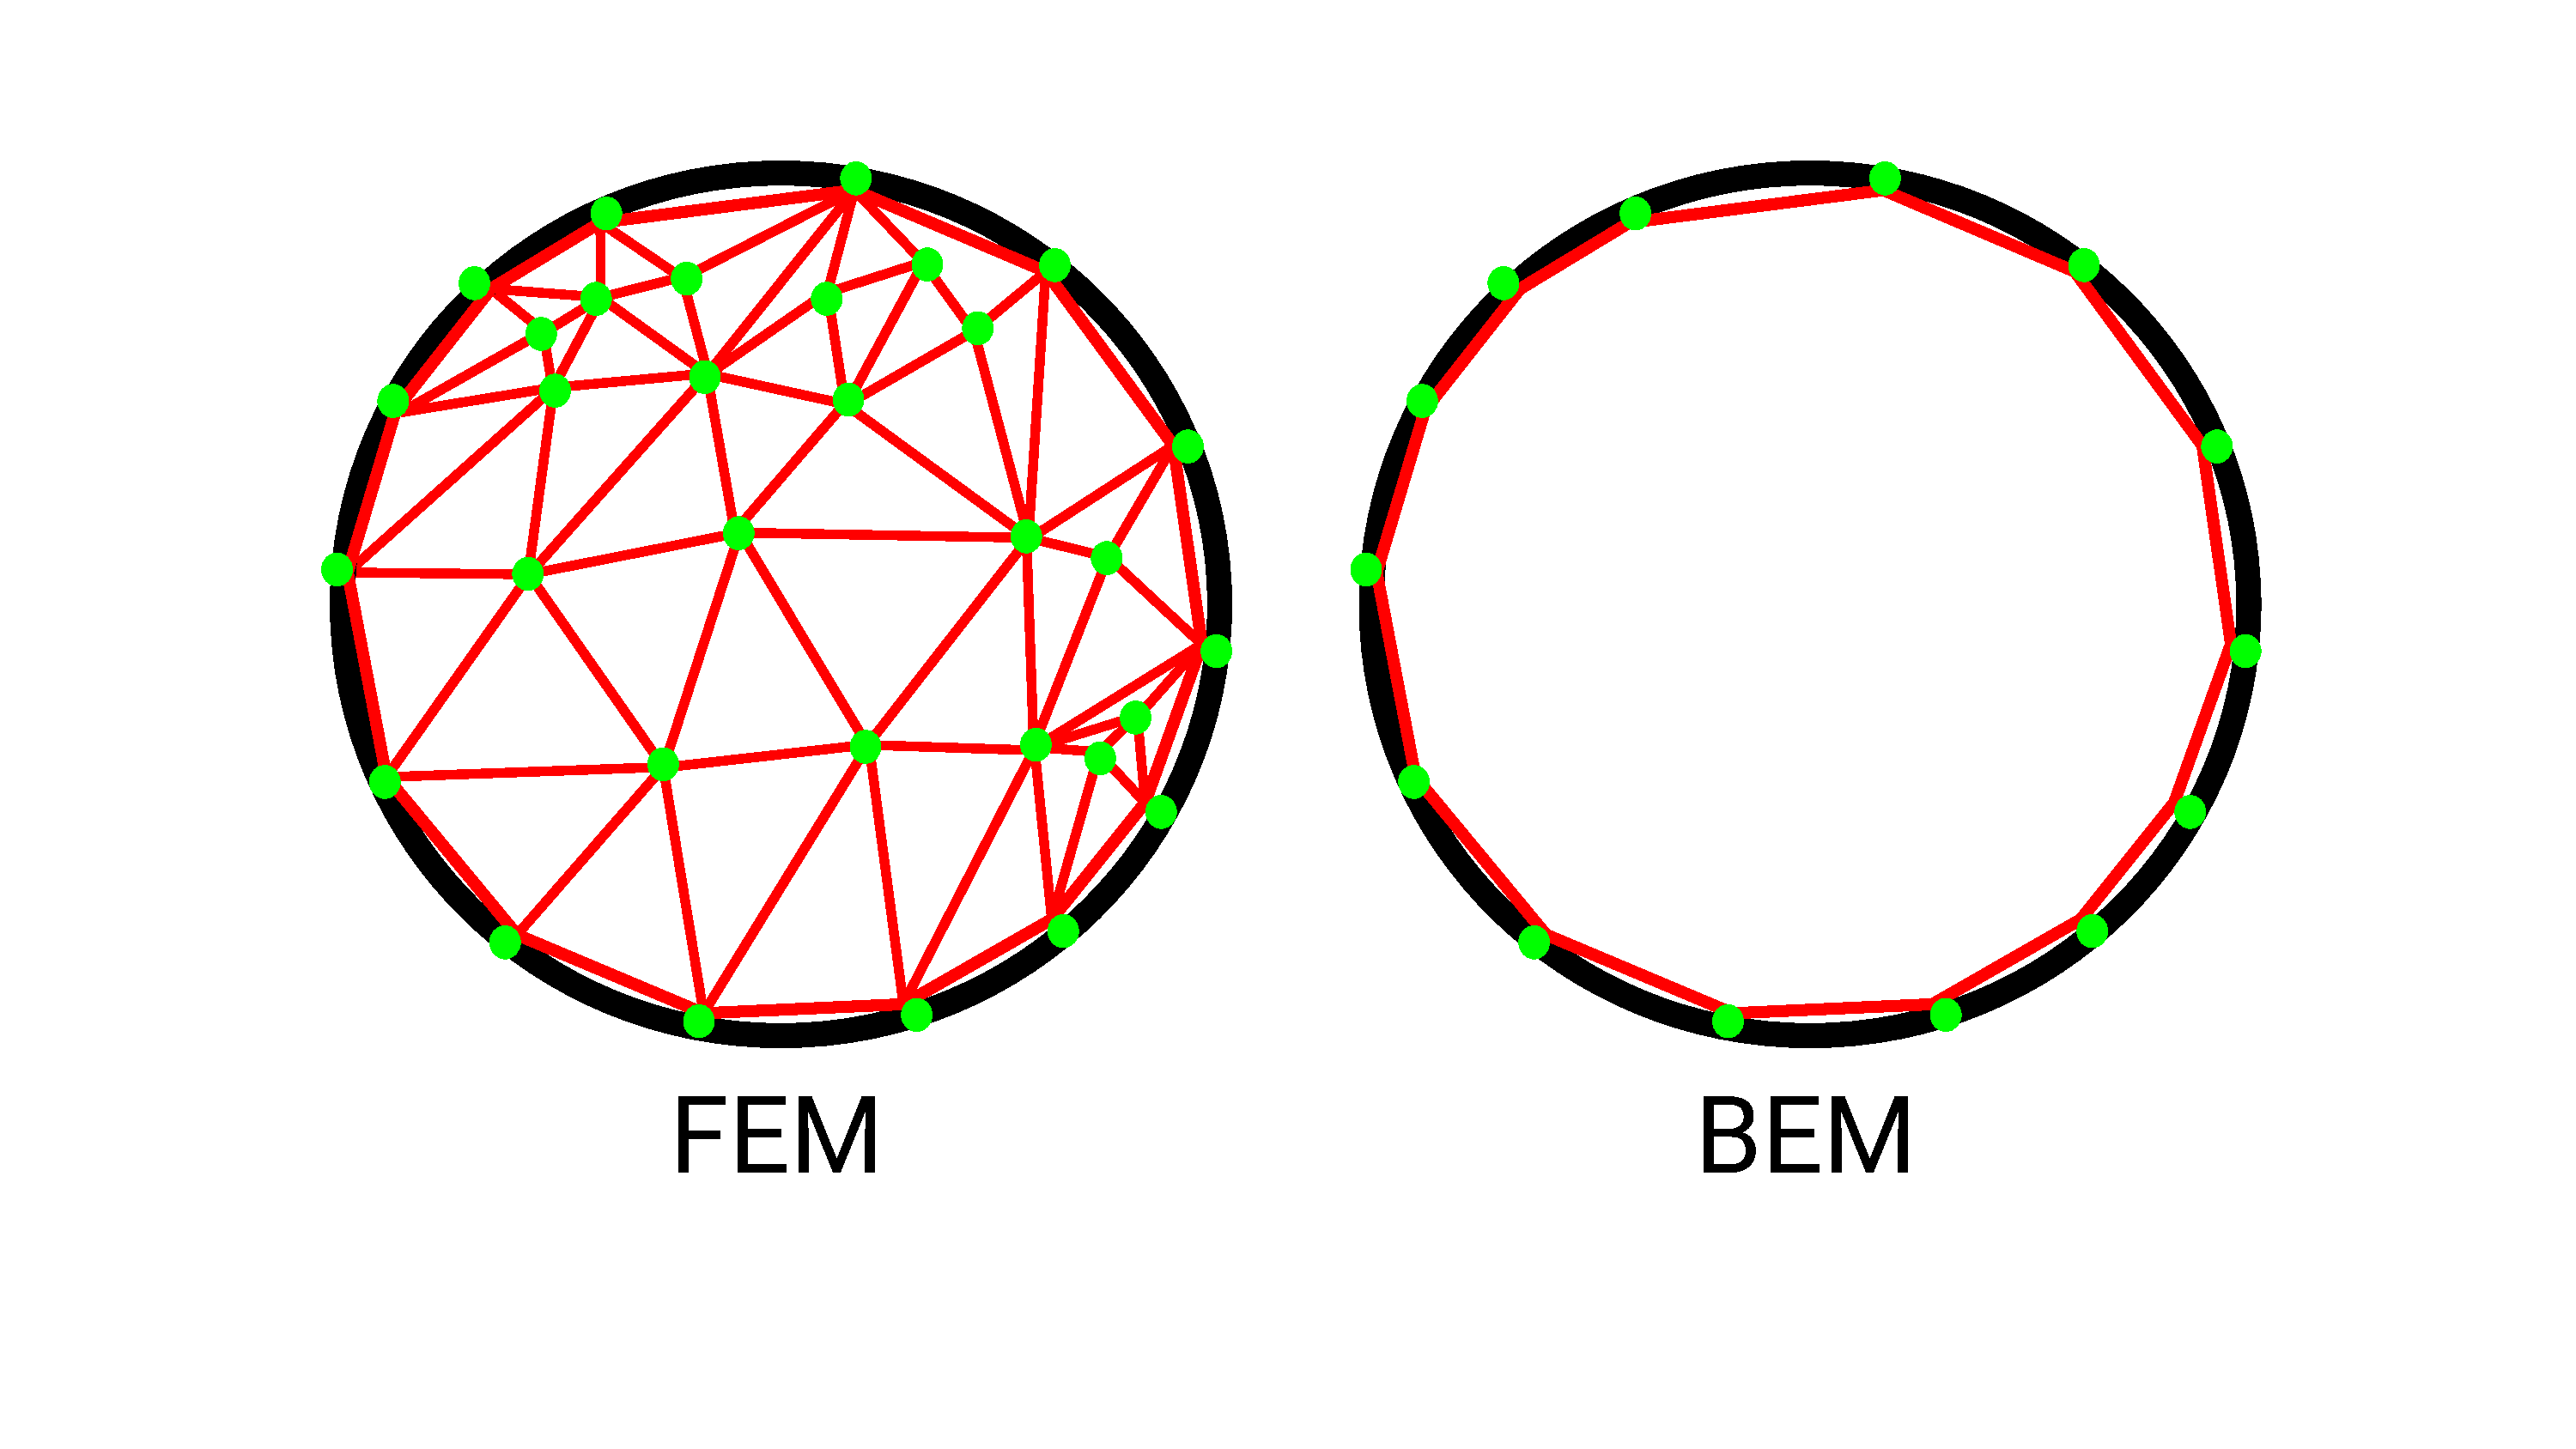
\includegraphics[width=\linewidth]{assets/fem_bem.pdf}
\end{frame}

\begin{frame}
    \frametitle{Laplace Interior Boundary Value Problem I}
    \begin{columns}
        \begin{column}{0.5\textwidth}

            Want to solve

            \begin{equation}
                \frac{\partial \phi}{\partial x^2} +  \frac{\partial \phi}{\partial y^2} = 0
            \end{equation}

            Inside a region of interest $\Omega$ which has some boundary $\partial \Omega$.


            \hspace*{5pt}

            We have conditions for the solution on the boundary:

            \begin{enumerate}
                    \item $\frac{\partial \phi(\partial \Omega)}{\partial n}$ - Neumann type.
                    \item $\phi(\partial \Omega)$ - Dirichlet type
            \end{enumerate}

        \end{column}

        \begin{column}{0.5\textwidth}

        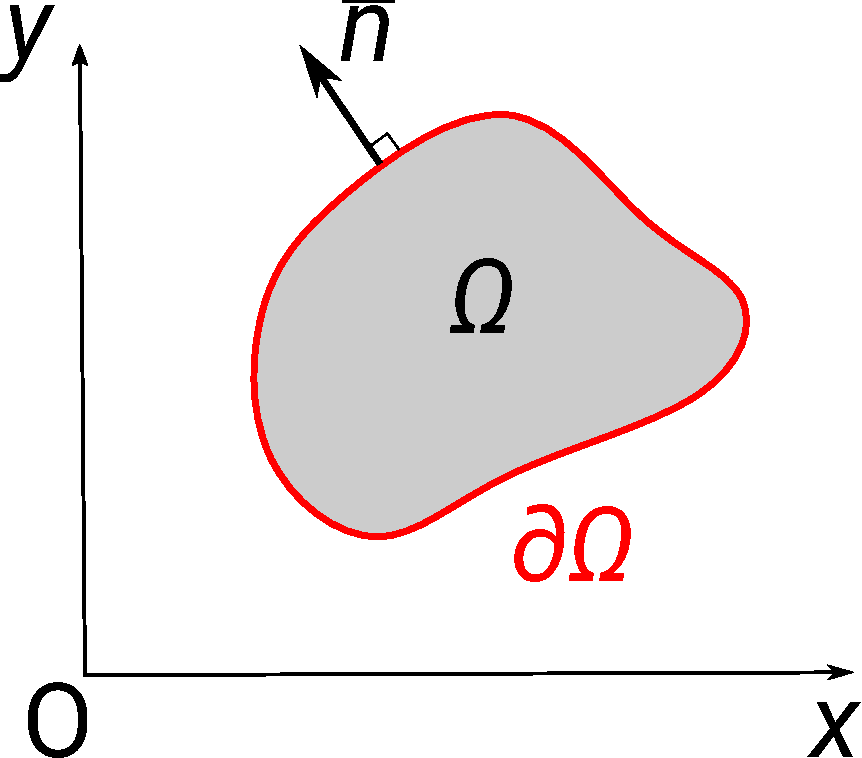
\includegraphics[width=\linewidth]{assets/laplace.pdf}
        \end{column}
    \end{columns}
\end{frame}

\begin{frame}
    \frametitle{Laplace Interior Boundary Value Problem II}

    Find a solution in terms of a \textit{boundary integral},

    \begin{equation}
        \begin{aligned}
        & \lambda(\xi, \eta)\phi(\xi, \eta) = \\
        &  \int_{\partial \Omega} [\phi(x, y) \frac{\partial}{\partial n}(\Phi(x, y; \xi, \eta)) - \Phi(x, y; \xi, \eta)\frac{\partial}{\partial n}(\phi(x, y))] ds(x, y)
        \end{aligned}
    \end{equation}

    Where,

  \begin{equation}
    \small
     \lambda(\xi, \eta) =
        \begin{cases}
          0 & (\xi, \eta) \notin \Omega \cup \partial \Omega\\
          1/2 & (\xi, \eta) \in \partial \Omega \\
          1 & (\xi, \eta) \in \Omega
        \end{cases}
    \end{equation}

  \hspace*{5pt}

  and the \textit{Fundamental Solution},

  \begin{equation}
    \small
    \Phi(x,y; \xi, \eta) = \frac{1}{4\pi} \ln [(x-\xi)^2 + (y-\eta)^2]
  \end{equation}

\end{frame}

\begin{frame}
    \frametitle{Laplace Interior Boundary Value Problem III}
    \begin{equation}
        \begin{aligned}
            & \lambda(\xi, \eta)\phi(\xi, \eta) = \\
            & \int_{\partial \Omega} [\phi(x, y) \color{red} \frac{\partial}{\partial n}(\Phi(x, y; \xi, \eta))  \color{black} - \color{red} \Phi(x, y; \xi, \eta) \color{black}\frac{\partial}{\partial n}(\phi(x, y))] ds(x, y)
        \end{aligned}
    \end{equation}
\end{frame}

\begin{frame}
    \frametitle{Laplace Interior Boundary Value Problem IV}

        Approximate with $N$ constant elements, with a midpoint value.

        \begin{equation}
            \begin{aligned}
                & \lambda(\xi, \eta)\phi(\xi, \eta) = \\
                & \sum_{k=1}^N  \overline{\phi(x, y)}^{(k)} \int_{\partial \Omega} \frac{\partial}{\partial n} (\Phi(x, y; \xi, \eta)) ds(x,y) \\
                &- \overline{\frac{\partial}{\partial n}(\phi(x, y))}^{(k)}  \int_{\partial \Omega} \Phi(x, y; \xi, \eta)  ds(x, y)
            \end{aligned}
        \end{equation}
\end{frame}

\begin{frame}
    \frametitle{Laplace Interior Boundary Value Problem V}
    \centering 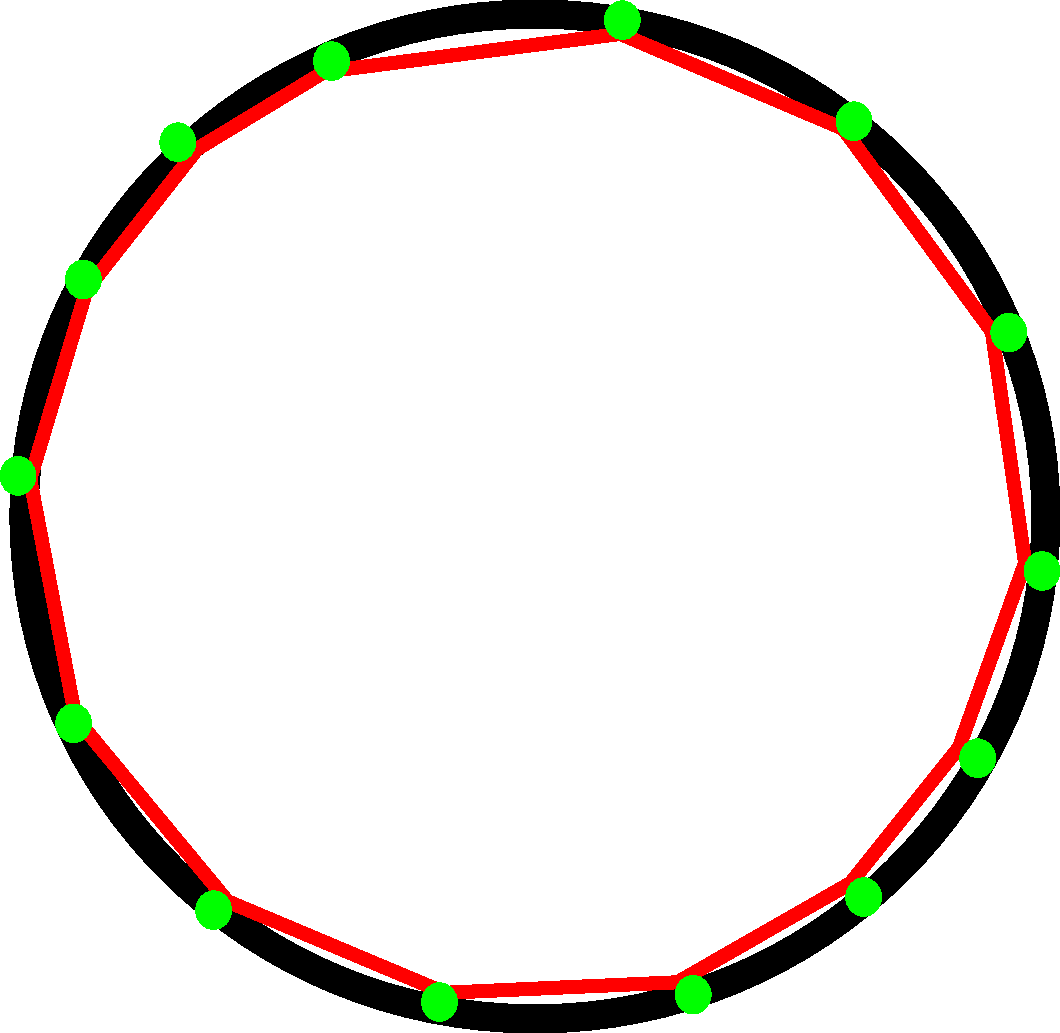
\includegraphics[width=0.5\linewidth]{assets/bem.pdf}
\end{frame}

\begin{frame}
    \frametitle{Laplace Interior Boundary Value Problem VI}

    Final Matrix Vector product (matvec) relating points on boundary, to solution in interior of the form,

    \begin{equation}
        Ax = b
    \end{equation}

    Where $A$ is the coefficient matrix, $x$ is the boundary data and $b$ is the solution.

    \begin{enumerate}
        \item $O(N^2)$ - $N$ elements.
        \item Poor scaling!
    \end{enumerate}
\end{frame}

\begin{frame}
    \frametitle{Fast Multipole Methods}
    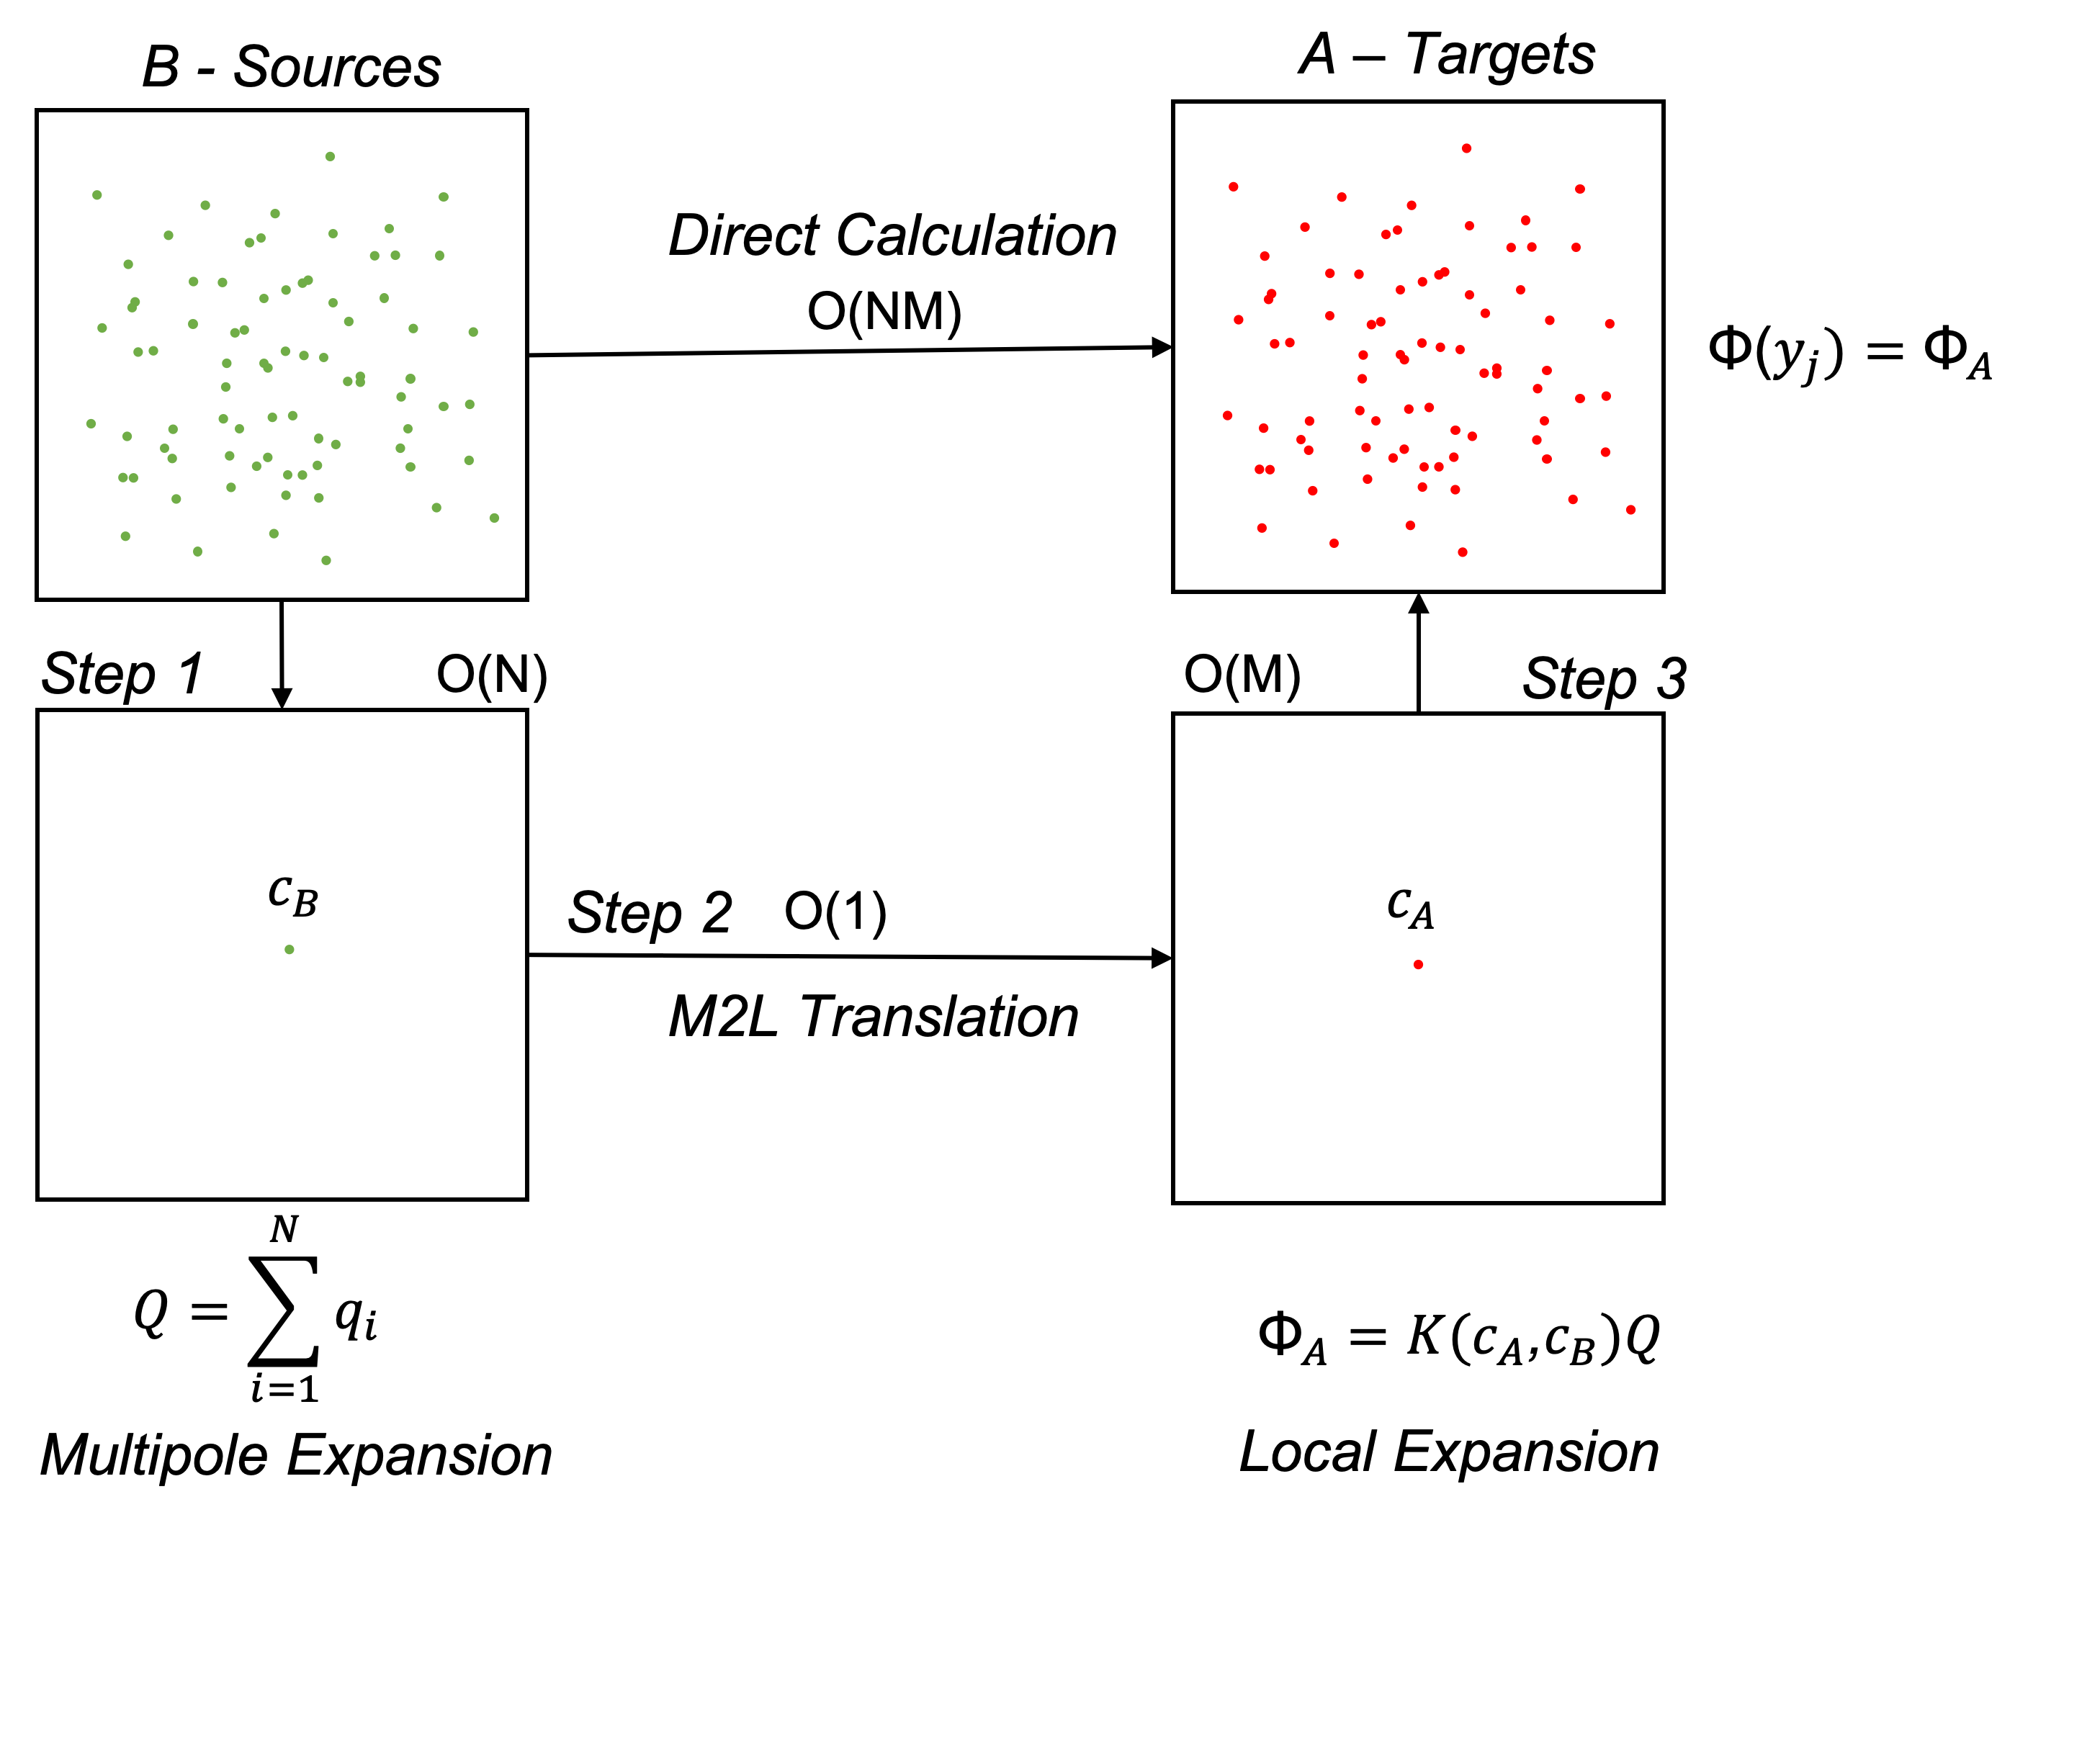
\includegraphics[width=\linewidth]{assets/three_step.png}
\end{frame}


\begin{frame}
    \frametitle{Fast Direct Solvers}
    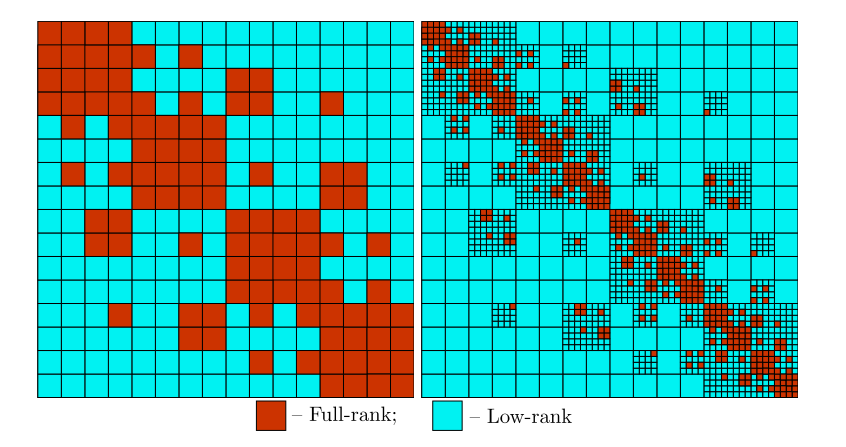
\includegraphics[width=\linewidth]{assets/ifmm.png}
    \captionof*{figure}{ \scriptsize Ambisekaran, S \& Darve, E. \textit{The Inverse Fast Multipole Method}, arXiv:1407.1572v1 (2014)}

\end{frame}

\begin{frame}
    \frametitle{Rusty Fast Solvers Project I}
    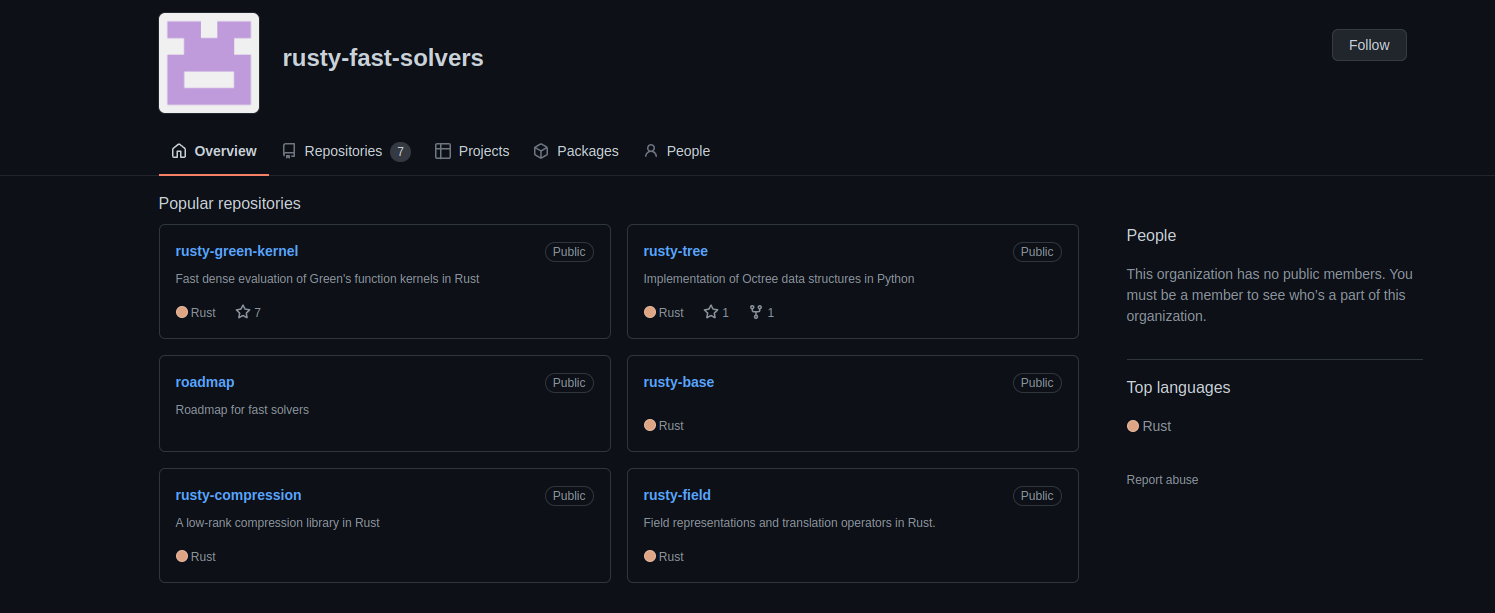
\includegraphics[width=0.95\linewidth]{assets/rfs.png}
    \captionof*{figure}{ \large https://github.com/rusty-fast-solvers}
\end{frame}

\begin{frame}
    \frametitle{Rusty Fast Solvers Project II}

    Checklist:

    \begin{enumerate}
        \item \color{green} Rusty Green Kernel  \color{black} - Optimized math kernel operations.
        \item \color{green} Rusty Tree \color{black} - Distributed Octrees.
        \item \color{green} Hyksort  \color{black} - Sorting algorithm for distributed arrays.
        \item \color{orange} Rusty Compression \color{black} - Randomized compression library.
        \item \color{orange} Rusty Field \color{black} - Field representations.
        \item \color{red} Rusty FMM \color{black} - Fast Multipole Method.
        \item \color{red} Rusty Inverse \color{black} - Fast Direct Solvers.
    \end{enumerate}

\end{frame}